\documentclass{article}

\usepackage{graphicx, amsmath}

% 0. Referencing style, APA-like referencing
\usepackage[backend=biber, style=apa, natbib=true]{biblatex}
\addbibresource{bibliography.bib} % Replace 'yourbibfilename.bib' with your actual .bib file name.

% 1.  Don't need such wide margins.
\usepackage[margin=1in]{geometry} % Setting the margins to 1 inch

\usepackage{amsmath}

\begin{document}

\title{Ordinal Data clustering and prediction}

\author{Quan Zhao}

\maketitle

\section{Introduction}


The study of ordinal data presents unique challenges and opportunities.
Ordinal data consists of categories with an inherent order but undefined
spacing. This makes it distinct from nominal and continuous data,
necessitating specialized analytical methods that acknowledge its
structured ordering without presuming equal intervals between its
categories.

This project investigates methods for clustering and predicting cluster
membership for ordinal data. These methods are useful because ordinal
data is prevalent in fields ranging from social sciences to healthcare.
We begin by defining ordinal data and describing its distinctive
features. We then discuss existing clustering and prediction
methodologies. We focus on model-based clustering because we have an
existing sophisticated approach of this type, that is tailored to the
ordinal nature of the data, whereas there are limitations inherent in
distance-based methods when applied to ordinal data. The report
describes specific statistical models developed for ordinal data
analysis, such as the Proportional Odds model and the Ordered Stereotype
Model, highlighting their effectiveness in extracting meaningful
insights.

We then reflect on the historical development of ordinal data analysis,
from early methodologies to recent innovations that have broadened its
applicability and improved its precision. We also consider future
research directions, including the potential for integrating machine
learning with conventional statistical methods to refine the predictive
performance of ordinal data models.

Clustering methods have previously been developed for ordinal data,
using models such as the Ordered Stereotype Model. However, these
existing methods do not include techniques for determining the likely
cluster membership of any new observations that were not available at
the initial clustering stage. Therefore, this research aims to extend
these existing methods to accurately predict cluster membership for
incoming data points. Such advancements are crucial for applying ordinal
data in dynamic environments where new data are produced frequently. The
accuracy of the predictions is also important, so we will assess this to
ensure that the methods perform sufficiently well.

In summary, this paper offers an examination of methodologies for
clustering and predicting ordinal data. This inquiry is intended as a
resource for both researchers and practitioners, providing insights
necessary for navigating the complexities of ordinal data and leveraging
its full potential in analytical endeavors.

\subsection*{Ordinal Data}

Ordinal data, a pivotal concept in statistical analysis, represents categorical data characterized by a meaningful order among its categories, without implying uniform differences between these ranks. Unlike nominal data, which merely categorizes without any implied ranking, ordinal data elevates the categorical analysis by introducing a hierarchy or sequence that is significant yet lacks quantifiable intervals between its elements. This characteristic distinguishes ordinal data: it conveys the sequence of values but remains silent on the magnitude of difference between successive ranks.

Such data often appear as rankings or ordered classifications where the precise distance between categories is undefined or irrelevant. 
Despite sometimes being numerically coded for analytical convenience, ordinal data resist traditional arithmetic operations, rendering calculations like addition or subtraction inappropriate and misleading.

In the realm of statistical analysis, ordinal data necessitates specialized, non-parametric methods. 
The median and mode stand out as appropriate measures of central tendency for this data types, 
aligning with their ordered nature without assuming equal intervals between categories.

Ordinal data's prevalence is notably high in social sciences, especially in surveys and questionnaires designed to capture subjective assessments such as attitudes, opinions, and preferences. These instruments frequently employ scales—ranging from ``strongly disagree'' to ``strongly agree''—to elicit responses that, while ordered, do not support the notion of fixed distances between adjacent categories. This principle underlines the core attribute of ordinal data: the clear hierarchy among responses without an inherent interval scale to quantify the gaps between them. Consequently, assigning numerical values to such categories for computational purposes is generally discouraged and conceptually flawed, as it misinterprets the data's ordinal nature 

(~\textcite{Johnson1999}) gives a good sample,
 It is typically rational to presume an order such as

 \[
 \text{strongly disagree} < \text{disagree} < \text{don’t know} < \text{agree} < \text{strongly agree}
\]
 However, it is often illogical to allocate integer values to these categories. Therefore, calculations like
\[
\text{``disagree''} - \text{``strongly disagree''}
\]

\[
\text{``agree''} - \text{``don't know''}
\]
are not considered valid. 
This demonstrates that performing arithmetic calculations on the numerical values assigned to the categories does not make sense.

\begin{figure}[ht!] % 'h!' places the figure here, in the text
    \centering % Centers the figure
    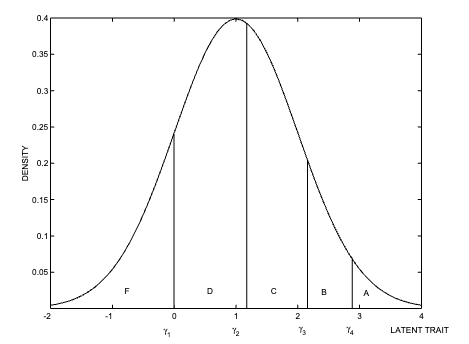
\includegraphics[width=0.6\textwidth]{images/ordinal_data_dist.png} % Include the image with 50% of the text width
    \caption{Latent trait interpretation of ordinal classification. 
    In this plot, the logistic density represents the distribution of latent traits for a particular individual. 
    It is assumed that a random variable is drawn from this density, and the value of this random variable determines an individual's classification. 
    For example, if a deviate of 0.5 is drawn, the individual receives a D. (~\cite{Johnson1999}).} % Caption for the image
    \label{fig:ordinal} % Label for referencing the figure in the text
  \end{figure}

\subsection*{Comparison with continuous numerical data}

In the context of statistical analysis, the distinction between ordinal and continuous numerical data types is pivotal, influencing both the choice of analytical methods and the depth of insights that can be derived. 
Ordinal data, characterized by its capacity to rank order categories without indicating precise differences between them, is inherently less informative than continuous numerical data. 
Continuous numerical data, with its quantitative nature, allows for an infinite range of values and supports detailed statistical operations, including arithmetic calculations and the application of advanced statistical models, facilitating a nuanced understanding of variables and their interrelations (~\cite{Stevens1946}).

The limitations of ordinal data stem from its inability to quantify the exact magnitude of differences between categories, a factor that restricts the application of parametric statistical methods. This constraint necessitates reliance on non-parametric methods, focusing on medians and modes rather than means and standard deviations, thereby offering a less detailed analysis (~\cite{Conover1999}). 
For instance, in Likert scale responses commonly used in surveys, the ordinal nature of data precludes meaningful calculations of averages or differences between responses, limiting the depth of analysis that can be achieved (~\cite{Likert1932}).

% task 7
Comparatively, continuous numerical data's capacity for precise measurement and the application of a broader range of statistical analyses enables a more detailed and accurate exploration of phenomena. 
This capability is contingent upon the availability of continuous numerical results, which may not always be feasible. The nature of the data collectible in certain research scenarios—such as measuring opinions, attitudes, or perceptions—often necessitates the use of ordinal data, due to the challenges associated with obtaining continuous measurements in these contexts. For instance, eliciting responses on a continuous percentage scale from 0 to 100 can be impractical when assessing subjective experiences or preferences. Hence, the decision to utilize ordinal data over continuous numerical data is not solely a matter of choice in research design and analysis but is also influenced by the practicalities of what data can realistically be gathered. This consideration is crucial for ensuring the validity and relevance of research findings, highlighting the importance of aligning data collection methods with the specific circumstances and constraints of the study.

In summary, while ordinal data is invaluable for capturing rankings and subjective assessments, 
its analytical limitations highlight the superior informational value of continuous numerical data in quantitative research. 
This distinction is crucial for researchers in the selection of appropriate statistical methods and in the interpretation of their data, 
ensuring that conclusions drawn are both valid and meaningful.

\subsection*{Clustering}

Clustering is a fundamental technique in the field of data analysis and machine learning, aimed at grouping a set of objects in such a way that objects in the same group (or cluster) are more similar to each other than to those in other groups. Its applications span a wide range of areas including market research, pattern recognition, image analysis, and bioinformatics, among others. For instance, in market research, clustering can help identify distinct customer segments based on purchasing behavior, while in bioinformatics, it can be used to classify different types of genes or proteins with similar functions.

There are primarily two types of clustering: distance-based clustering and model-based clustering.

1. \textbf{Distance-based Clustering}: This approach relies on the concept of similarity or distance between data points. The aim is to minimize the distance between data points within a cluster while maximizing the distance between data points in different clusters. Popular methods include K-means, hierarchical clustering, and DBSCAN, each using different metrics (e.g., Euclidean, Manhattan) to measure distance or similarity.

2. \textbf{Model-based Clustering}: Unlike distance-based methods, model-based clustering assumes that the data is generated from a mixture of finite distributions, where each component of the mixture represents a cluster. This approach tries to estimate the parameters of these distributions to optimize the fit between the model and the data. Model-based methods are particularly useful for complex data structures, including those with mixed types of data (numerical, categorical) or where the clusters have different sizes, shapes, or orientations.

Model-based clustering is often more suitable for ordinal data—data that contain natural, orderable categories. This is because ordinal data, which embody an inherent ranking or order (e.g., survey responses from "strongly agree" to "strongly disagree"), do not fit well with the distance metrics used in distance-based clustering, which treat distances between all pairs of categories as equal. Model-based clustering, on the other hand, can accommodate the ordinal nature by incorporating it into the model assumptions, allowing for a more nuanced understanding and grouping based on the inherent order of the data. This method can capture the ordinal information effectively, providing more meaningful and interpretable clusters for analysis.

\section{Statistical-based Ordinal Data Clustering}

\subsection{Finite Mixture modeling}

Finite mixture models have emerged as a versatile and powerful statistical tool, garnering increasing attention across various scientific and research disciplines. These models, predicated on the assumption that observed data arise from a blend of several probability distributions, each representing a distinct subpopulation, have revolutionized our approach to understanding complex data structures. The designation ``finite'' in finite mixture models is pivotal, indicating the specific, but variable, number of components or subgroups within the data. This finite aspect offers a balance between model complexity and interpretability, allowing for detailed yet manageable analysis of diverse datasets.

The Finite mixture model is defined as:
\begin{equation}
p(x_i|\mathbf{\Theta}) = \sum_{k=1}^{K} \pi_k f(x_i|\theta_k)
\end{equation}
where:
\begin{itemize}
    \item $p(x_i|\mathbf{\Theta})$ denotes the overall mixture model's density or mass function for observation $x_i$.
    \item $K$ is the total number of component distributions in the mixture.
    \item $\pi_k$ represents the mixing proportion of the $k$th component, satisfying $0 \leq \pi_k \leq 1$ and $\sum_{k=1}^{K} \pi_k = 1$.
    \item $f(x_i|\theta_k)$ is the probability density function (pdf) or probability mass function (pmf) of the $k$th component distribution evaluated at $x_i$.
    \item $\theta_k$ denotes the parameter vector of the $k$th component distribution.
    \item $\mathbf{\Theta}$ symbolizes the complete set of parameters for the mixture model, including both the mixing proportions $\{\pi_1, \ldots, \pi_K\}$ and the parameters of the component distributions $\{\theta_1, \ldots, \theta_K\}$.
\end{itemize}

The significance of finite mixture models is vividly illustrated in Figure~\ref{fig:trend}, which showcases a robust upward trajectory in related publications. This trend not only reflects the growing academic and practical interest in these models but also underscores their evolving sophistication and broadening applicability. From the early advancements in maximizing likelihood estimation through algorithms like EM, as pioneered by McLachlan in 2000, to the more recent developments in handling a variety of data types, including binary, count, and ordinal data, finite mixture models have continuously adapted and expanded their scope.

\begin{figure}[ht!] % 'h!' places the figure here, in the text
    \centering % Centers the figure
    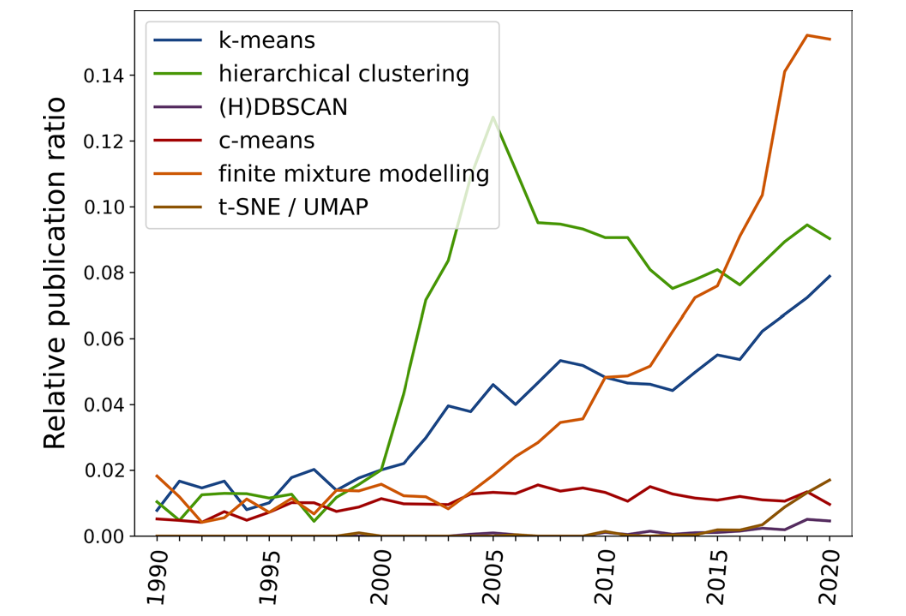
\includegraphics[width=0.6\textwidth]{images/trend.png} % Include the image with 50% of the text width
    \caption{The increase in publications indexed by PubMed that mention a keyword specific to cluster analyses relative to the number of publications 
    that mention a traditional statistical test. 
    Particularly sharp increases can be seen for finite mixture modelling.
    From~\cite{dalmaijer2022statistical}.} % Caption for the image
    \label{fig:trend} % Label for referencing the figure in the text
  \end{figure}

\subsection{Proportional Odds model}

The Proportional Odds model (~\cite{mccullagh1980regression}) is another approach which defined for an ordinal response variable $Y$ with $K$ ordered categories ($k=1, 2, \ldots, K$). 
The model expresses the cumulative log odds of $Y$ being less than or equal to a category $k$ as follows:

\begin{equation}
log(P(Y \leq k )) = \mu_k - \alpha_g
\end{equation}

where:
\begin{itemize}
    \item $P(Y \leq k)$ is the cumulative probability of $Y$ being in category $k$ or any category below $k$.
    \item $\mu_k$ is the intercept term for category $k$, which allows the log odds to vary across categories.
    \item $\alpha_g$ represents the effects cluster $g$ and $C$ with clusters ({$g=1, 2, \ldots, G$}).
    \item The model assumes that the effect of the predictors on the log odds of being in a lower versus a higher category is proportional across all categories.
\end{itemize}

\subsection{Ordered Stereotype Regression Model}

The Ordered Stereotype Regression Model  (~\cite{anderson1984regression}) is a statistical approach designed to analyze ordinal dependent variables, where the outcomes are categories with a natural order but not a quantifiable difference between them.

Given an ordinal response variable $Y$ with categories ($k=1, 2, \ldots, K$) the probability of $Y$ falling into the $k$th category, is denoted as $P(Y = k)$.


The logit for category $k$ is then:
\begin{equation}
log\left(\frac{P(Y = k)}{P(Y = 1)}\right) = \mu_k + \phi_k \alpha_g
\end{equation}

where $\mu_k$ is the intercept for category $k$, 
and $\alpha$ represents the effects cluster $g$, where $g \in C$.
And come with hypothesis
$0 = \phi_1 \leq \phi_2 \leq \ldots \leq \phi_K = 1.$
Stereotype model is unconstrained, $\phi$ add restricts to make it works for ordinal data.
This allows the effects to vary across categories but constrains them to follow a scaled version of a common pattern.

% 123

\subsection{Expectation-Maximization (EM) Algorithm}

% EM algorithm has been introduced by Dempster, Laird and Rubin in 1977. (~\cite*[Dempster, Laird and Rubin]{Dempster1977}).

% The Expectation-Maximization (EM) algorithm is a two-step iterative method to obtain the maximum likelihood estimate (MLE) of the parameters of a statistical model, where the model depends on unobserved latent variables. The EM algorithm is particularly useful for mixture models, where the data is considered to be generated from a combination of several different statistical distributions, each representing a different 'component' of the population.

% \subsubsection*{Expectation-Maximization Algorithm for Mixture Model}

% A mixture model is a probabilistic model for representing the presence of subpopulations within an overall population, without requiring that an observed data set explicitly identify the subpopulation to which an individual observation belongs. Formally, if we assume a mixture of $K$ components, the probability density function (pdf) of a mixture model can be written as:

% \begin{equation}
% p(x|\Theta) = \sum_{k=1}^{K} \pi_k f_k(x|\theta_k)
% \end{equation}

% where $x$ represents the data points, $\Theta$ represents the parameters of the mixture model which include both the mixing coefficients $\pi_k$ and the parameters of the component distributions $\theta_k$, $f_k$ is the component distribution, and $\pi_k$ are the mixing coefficients such that $\sum_{k=1}^{K} \pi_k = 1$ and $\pi_k \ge 0$.

% \subsubsection{Introduction to the EM Algorithm}
The Expectation-Maximization (EM) algorithm is a powerful statistical tool for finding maximum likelihood estimates in models with latent variables. It consists of two main steps: the Expectation step (E-step) and the Maximization step (M-step).

During the E-step, the algorithm estimates the expected value of the log-likelihood function, with respect to the conditional distribution of the latent variables given the observed data and the current estimates of the parameters. This step can be formally expressed as follows:
\begin{equation}
Q(\theta | \theta^{(t)}) = E_{Z|X,\theta^{(t)}}[\log L(\theta; X, Z)]
\end{equation}
where \( \theta \) denotes the parameter vector, \( X \) represents the observed data, \( Z \) are the latent variables, \( L \) is the likelihood function, and \( \theta^{(t)} \) are the parameter estimates from the previous iteration.

In the M-step, the algorithm maximizes the expected log-likelihood found in the E-step with respect to the parameters to obtain new parameter estimates:
\begin{equation}
\theta^{(t+1)} = \arg \max_{\theta} Q(\theta | \theta^{(t)})
\end{equation}

\subsubsection*{E-step (Expectation Step)}

During the Expectation step, the EM algorithm computes the expected value of the log likelihood function, with respect to the conditional distribution of the latent variables given the observed data under the current estimate of the parameters. This step involves calculating the posterior probabilities that a given data point belongs to each of the $K$ components, based on the current estimates of the parameters.

For a mixture model, the posterior probability (also known as the responsibility) that component $k$ generates data point $x_i$ is calculated as:

\begin{equation}
\gamma(z_{ik}) = \frac{\pi_k f_k(x_i|\theta_k)}{\sum_{j=1}^{K} \pi_j f_j(x_i|\theta_j)}
\end{equation}

where $\gamma(z_{ik})$ is the responsibility that component $k$ has for data point $i$.

\subsubsection*{M-step (Maximization Step)}

In the Maximization step, the EM algorithm updates the parameters of the model to maximize the expected log likelihood found in the E-step. 
This involves updating the estimates of both the parameters of the component distributions and the mixing coefficients.

Update the mixing coefficients:

\begin{equation}
\pi_k^{new} = \frac{1}{N} \sum_{i=1}^{N} \gamma(z_{ik})
\end{equation}

% 2. Update the parameters of the component distributions ($\theta_k$), which depends on the form of the distribution. For example, in a Gaussian mixture model, the mean and covariance of each Gaussian component are updated as follows:

% \begin{equation}
% \mu_k^{new} = \frac{\sum_{i=1}^{N} \gamma(z_{ik}) x_i}{\sum_{i=1}^{N} \gamma(z_{ik})}
% \end{equation}

% \begin{equation}
% \Sigma_k^{new} = \frac{\sum_{i=1}^{N} \gamma(z_{ik}) (x_i - \mu_k^{new})(x_i - \mu_k^{new})^T}{\sum_{i=1}^{N} \gamma(z_{ik})}
% \end{equation}

% where $N$ is the total number of data points.

% abc

% \section{Expectation-Maximization Algorithm for Clustering in Finite Mixture Models}



\subsection{EM Algorithm Sample for clustering by Ordered Stereotype Regression Model}
For clustering within a finite mixture model, the EM algorithm treats the cluster assignments as latent variables. The objective is to maximize the likelihood of the observed data under the mixture model.

The E-step computes the posterior probabilities that an observation belongs to each cluster, given the current parameter estimates. This can be expressed for a particular cluster \( k \) as follows:
\begin{equation}
P_{ij}(Y_{ij} = k) = \frac{e^{\mu_k + \phi_k \cdot x_r}}{\sum_{q=1}^{Q} e^{\mu_q + \phi_q \cdot x_r}}
\end{equation}
where \( P_{ij} \) denotes the probability that the \( i \)-th observation in the \( j \)-th cluster is in cluster \( k \), \( \mu_k \) and \( \phi_k \) are the current estimates of the parameters for cluster \( k \), and \( x_r \) represents the observed data.

The M-step then updates the parameter estimates to maximize the likelihood given the posterior probabilities computed in the E-step. The new parameter estimates for cluster \( k \) are computed as:
\begin{equation}
\theta_{k}^{(t+1)} = \frac{\sum_{i=1}^{N} P_{ij}(Y_{ij} = k) \cdot x_{i}}{\sum_{i=1}^{N} P_{ij}(Y_{ij} = k)}
\end{equation}
where \( N \) is the number of observations, and \( x_{i} \) is the observed data for the \( i \)-th observation.

The algorithm iterates between these two steps until the change in the likelihood or the parameter estimates is below a pre-defined threshold, indicating convergence.

% efg


\section{History of Statistical based Ordinal Data Clustering}

\subsection*{Early Developments (2000--2010)}

McLachlan \& Basford 1988 (~\cite{mclachlan1988mixture}) start to marked a crucial step in mixture model applications by simplifying the maximum likelihood estimation (MLE) using the EM algorithm.

McLachlan \& Peel's 2000 book further elaborate on this approach. This approach, utilizing $Y_j$ and $Z_j$, not only enhanced the computational efficiency of MLE but also laid a foundational strategy for Bayesian approaches and MCMC methods in mixture models. The paper’s impact is evident in its widespread adoption across various domains, from bioinformatics to finance, where mixture models are employed (~\cite{mclachlan2000finite}).

In 2002, Figueiredo's introduction of an unsupervised algorithm for learning finite mixture models was a game-changer. This method's ability to autonomously select the number of components represented a significant leap over previous techniques, which often relied on arbitrary or manual component selection. Additionally, the algorithm's robustness against initialization issues and singular estimates made it a go-to choice for practitioners dealing with complex multivariate data (~\cite{figueiredo2002unsupervised}).

A key paper in 2010 by Volodymyr and Ranjan addressed practical challenges in applying the EM algorithm for mixture models. This comprehensive guide to estimation, model selection, and likelihood maximization was a boon for both researchers and practitioners. Notably, the work extended beyond Gaussian mixtures, offering insights and methodologies for simulating and visualizing non-Gaussian mixtures, thereby broadening the applicability of mixture models (~\cite{10.1214/09-SS053}).

\subsection*{Recent Developments (2010--2019)}

In 2016, Matechou et al. introduced a novel approach to data analysis with their proposal of finite mixture models for biclustering two-mode ordinal categorical data. Utilizing proportional odds parameterization, these models offered a sophisticated understanding of complex data patterns, particularly beneficial in fields such as genomics and social sciences where ordinal data is prevalent. The application of the EM algorithm for model fitting highlighted the continued importance of this method in the context of mixture model applications (~\cite{matechou2016biclustering}).

Similarly, in 2016, Fernandez et al. presented an alternative methodology for clustering ordinal data by employing likelihood-based methods through finite mixtures with the stereotype model. This approach stood out for its use in fuzzy clustering techniques, an area that has been attracting increased attention in the realm of data science (~\cite{fernandez2016mixture}).

In 2019 Fernandez et al.'s extension of finite mixture models to binary, count, and ordinal data under a unified statistical framework represented a consolidation and expansion of mixture model applications. The introduction of maximum likelihood estimation parameters and the Bayesian approach for simultaneous estimation were indicative of the field's progression towards more flexible and comprehensive modeling techniques (~\cite{fernandez2019finite}).

The primary innovation in both of these studies lies in the integration of ordinal data models with finite mixture methods, a departure from the traditional use of finite mixtures for continuous variables.


Jacques and Biernacki's 2018 introduction of a model-based co-clustering algorithm was a significant advancement. The algorithm's ability to handle missing data and its interpretability made it especially relevant for high-dimensional datasets. The BOS distribution employed in this model underscored the continuous innovation in probabilistic modeling techniques, catering to the increasing complexity of data in modern research (~\cite{jacques2018model}).

Compare with previous work, Jacques and Biernacki's (~\cite{jacques2018model}) method is based on a novel Binary Ordinal Search (BOS) model emphasizing efficiency and interpretability, especially with missing data. 

\subsection*{Compare with other clustering algorithm}

Compared to tree based or distance based clustering algorithms, statistical based clustering algorithms demonstrate superior performance with ordinal data, particularly in scenarios involving multiclass and multioutput cases. 
This advantage stems from two key factors: firstly, ordinal data do not presuppose equal distances between categories, a condition that distance-based methods often rely on. Secondly, ordinal data typically encompass only a few categories, which can limit the effectiveness of tree-based methods designed to partition data across a broader numerical range.

\section{Cluster Prediction for Ordinal Data}

This project uses finite mixture models to predict cluster membership for ordinal data. We will make use of existing clustering methods to cluster ordinal data, and then we will propose a new method for predicting the membership for new observations. We use the Ordered Stereotype Model (OSM) for ordinal data, because it is parsimonious but flexible.
Whilst we will focus in this project on this particular model and this particular type of data, the general approach we propose can be applied to other finite mixture models that are tailored to fit other data types. Our method can also be adapted to cluster the variables of the dataset instead of the observations, because we extend an existing clustering approach that can perform both of those tasks. Thus this study not only introduces a robust cluster prediction approach but also sets the stage for future explorations ordinal data analysis.

\subsection{Methodological Overview}

The essence of our approach lies in leveraging the estimates obtained from the Expectation-Maximization (EM) algorithm, which provides us with crucial parameters ($\mu$, $\phi$, and $\alpha$) necessary for the prediction process. Specifically, within the framework of the OSRM, the EM algorithm's M-step furnishes us with estimates for the intercepts ($\mu$) and the effects ($\phi$ and $\alpha$) for each category ($k$), thereby laying the groundwork for predicting cluster membership.

Given a new ordinal response variable $\tilde{Y}$, the probability that an observation belongs to a particular cluster ($g$) is articulated as follows:

\begin{equation}
P(C=g|\tilde{Y}=k) = \mu_k + \phi_k \alpha_g
\end{equation}

This formula serves as the cornerstone for our predictive framework, enabling a nuanced understanding of how new data points correlate with existing clusters.

\subsection{Practical Implementation}

In practice, the predictive model begins with a dataset randomly partitioned into two subsets: $Y$ for training and $\tilde{Y}$ for validation. The training set, $Y$, is utilized to calibrate the regression model—yielding estimates for the parameters $\mu$, $\phi$, and $\alpha$ through the application of the EM algorithm. Subsequently, for each instance within the $\tilde{Y}$ set, the model computes the probability of cluster membership based on the established parameters, thereby facilitating the prediction of cluster assignments for new observations.

This pragmatic approach underscores the model's adaptability and its capacity to handle real-world data complexities, offering a robust tool for predictive clustering in various domains.

\subsection{Application Context and Datasets}

The practical utility of our cluster prediction method is exemplified through its application to the Public Sector Commission WA Employee Perception Survey 2016. Conducted by the Public Sector Commission of Western Australia, this survey gathered insights into employee perceptions on pivotal workplace factors, such as leadership dynamics, communication efficacy, and the balance between work and life. The survey's findings are instrumental in deciphering the nuances of organizational culture and pinpointing potential areas for enhancement within the public sector.

The 2016 iteration of the survey witnessed participation from employees across 11 public sector entities, boasting a response rate of 53\% and culminating in 3,883 valid responses. This dataset, encompassing individual responses, the survey instrument, and a summary of results, is disseminated under the Creative Commons Attribution 3.0 Australia license, providing a rich resource for analysis and application of the discussed predictive clustering approach.

\section{Conclusion and Future Directions}

The evolution of mixture models from the foundational work of McLachlan in 2000 to the advanced developments up to 2019 exemplifies a trajectory marked by significant growth and innovation. These advancements have not only addressed longstanding challenges but also paved the way for future breakthroughs. A critical aspect of this ongoing evolution is the integration of machine learning with traditional statistical methods, enhancing the predictive accuracy of cluster memberships for new data points—a capability increasingly vital in fields such as artificial intelligence, where precision in pattern recognition and decision-making is paramount.

The proposed methodology for cluster prediction in ordinal data, integrating finite mixture models with regression analysis, signals a pivotal advancement in the statistical analysis domain. Our plan to utilize the Public Sector Commission WA Employee Perception Survey 2016 as a benchmark to evaluate the performance of this approach underscores our commitment to rigorous empirical validation. This dataset serves as a crucial testbed for demonstrating the method's effectiveness in navigating the intricacies of ordinal data and its potential for broad applicability across diverse research areas.

As we advance, the growing complexity and volume of data underscore the need for models that are robust, efficient, and adaptable to a wide range of data types and structures. Future research will focus on enhancing these models' scalability and adaptability, further refining their predictive capabilities across increasingly complex datasets. This forward-looking agenda aims to solidify the role of mixture models in modern data analysis, ensuring they remain indispensable tools capable of confronting the expanding challenges in data science and artificial intelligence. Embracing the confluence of traditional statistical techniques and modern machine learning methodologies, mixture models are set to drive the next wave of innovations in data exploration, offering new insights and enhanced analytical capabilities.

\printbibliography

\end{document}
